% !TEX root = SegwayDoku.tex
\renewcommand{\autoren}{Valentyn Chepil, Alexsander Stoiljkovic}
\newpage
\section{Die Gehäuse}
\subsection{Die Gehäusen - V.1}
% \ref{bild_3} zuweisung auf Bild in Text.

\begin{figure}[!h]  % [h] bedeutet, dass das Bild genau an dieser Stelle im Text erscheint
	% mit width=... wird die Größe des Bildes in Prozent der Seitenbreite eingestellt
	\centering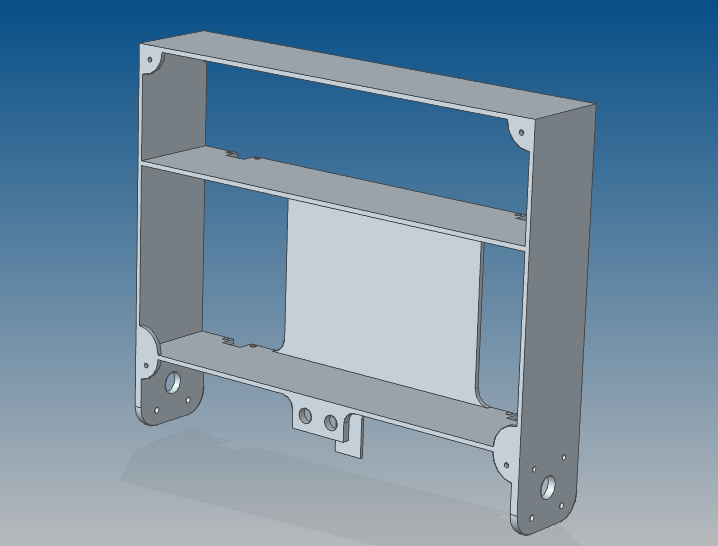
\includegraphics[width=0.5\textwidth]{images/gehaeuse-v1.png}
	% caption ist die Bildunterschrift, taucht auch im Abbildungsverzeichnis auf
	\caption{Gehäuse - V.1 \newline (Quelle: eigene Darstellung)}
	\label{gehaeuse-v1} % über das label kann man aus dem Text auf das Bild verweisen
\end{figure}

\subsection{Die Gehäusen - V.2}
Modul Aufbau: ....
% Text einfügen, dass Herr Nitsche zuerst einfache Gehäuser wollte, danach kam vorschlag Mogulaufbau machen.

\begin{figure}[!h]  % [h] bedeutet, dass das Bild genau an dieser Stelle im Text erscheint
	% mit width=... wird die Größe des Bildes in Prozent der Seitenbreite eingestellt
	\centering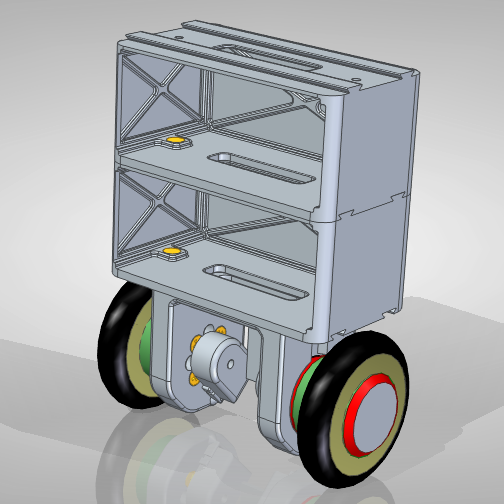
\includegraphics[width=0.5\textwidth]{images/gehaeuse-v2.png}
	% caption ist die Bildunterschrift, taucht auch im Abbildungsverzeichnis auf
	\caption{Gehäuse - V.2 \newline (Quelle: eigene Darstellung)}
	\label{gehaeuse-v2} % über das label kann man aus dem Text auf das Bild verweisen
\end{figure}
% Modul, Motorhalter ansichten zeigen und Text.
\begin{figure}[!h]  % [h] bedeutet, dass das Bild genau an dieser Stelle im Text erscheint
	% mit width=... wird die Größe des Bildes in Prozent der Seitenbreite eingestellt
	\centering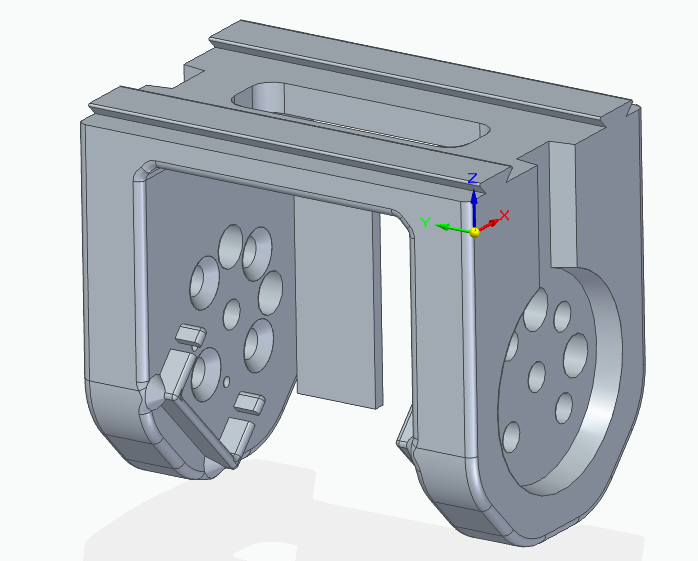
\includegraphics[width=0.5\textwidth]{images/MH.png}
	% caption ist die Bildunterschrift, taucht auch im Abbildungsverzeichnis auf
	\caption{Endgültige Gehäuse - V.3 \newline (Quelle: eigene Darstellung)}
	\label{MH} % über das label kann man aus dem Text auf das Bild verweisen
\end{figure}

\subsection{Die Gehäusen - V.2}
Modul Aufbau: ....

% Text einfügen, dass nach lange Beschprechungs mit Herr Nitsche kam eune endgültige Gehäuser.

\begin{figure}[!h]  % [h] bedeutet, dass das Bild genau an dieser Stelle im Text erscheint
	% mit width=... wird die Größe des Bildes in Prozent der Seitenbreite eingestellt
	\centering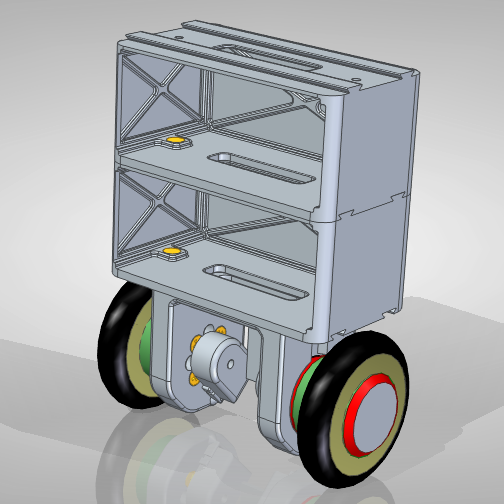
\includegraphics[width=0.5\textwidth]{images/gehaeuse-v2.png}
	% caption ist die Bildunterschrift, taucht auch im Abbildungsverzeichnis auf
	\caption{Gehäuse - V.2 \newline (Quelle: eigene Darstellung)}
	\label{gehaeuse-v3} % über das label kann man aus dem Text auf das Bild verweisen
\end{figure}

%\begin{figure}[!h]  % [h] bedeutet, dass das Bild genau an dieser Stelle im Text erscheint
	% mit width=... wird die Größe des Bildes in Prozent der Seitenbreite eingestellt
%	\centering\includegraphics[width=0.5\textwidth]{images/123.png}
	% caption ist die Bildunterschrift, taucht auch im Abbildungsverzeichnis auf
%	\caption{Endgültige Gehäuse - V.3 \newline (Quelle: eigene Darstellung)}
%	\label{MH123} % über das label kann man aus dem Text auf das Bild verweisen
%\end{figure}

\pagebreak
